\chapter{Metode}

\section{Udviklingsværktøjer}

\subsection{Analyse og designmetode}

Dette afsnit har til formål at beskrive hvilke tekniske metoder, der er benyttet af udarbejdelsen af bachelorprojektet. Primært er der tale om metoder fra faget ISE. I dette afsnit bliver der også beskrevet hvilke arbejdsredskaber, der er benyttet til udførelse af bachelorprojektet og rapporten.\\

Udviklingsforløbet er udarbejdet efter V-modellen og ASE-modellen \cite{IngeniorhojskolenAarhusUniversiteta} som er udviklet af Aarhus Ingeniørskole. ASE-modellen anvendes til udvikling af software og hardware, som er delt op i faser. For hver fase kommer en række artefakter som tilsammen resulterer i et veldokumenteret bachelorprojekt. Disse faser kombineres med V-modellen. I dette bachelorprojekt er der udført modultest på alle moduller opført i både hardware og software. Efter at kunne godkende modultestene, er en integrationstest blevet udført, hvor det bygget hardware og software er sammensat og testet som et samlet system. Her gøres det klart at systemet fungerer som intentionen, inden accepttesten nåes. Accepttesten er undersøger om alle krav i specificeret i kravspecifikationen er overholdt. Vejleder, Thomas Nielsen, lærer ved Aarhus Ingeniør Højskole, har deltaget i udførelsen af accepttesen, godkendt og underskrevet den. 
Brugen af ASE-modellen og kombinationen af V-modellen har resulteret i denne veldokumenteret rapport.   

\begin{figure}[H]
\centering
{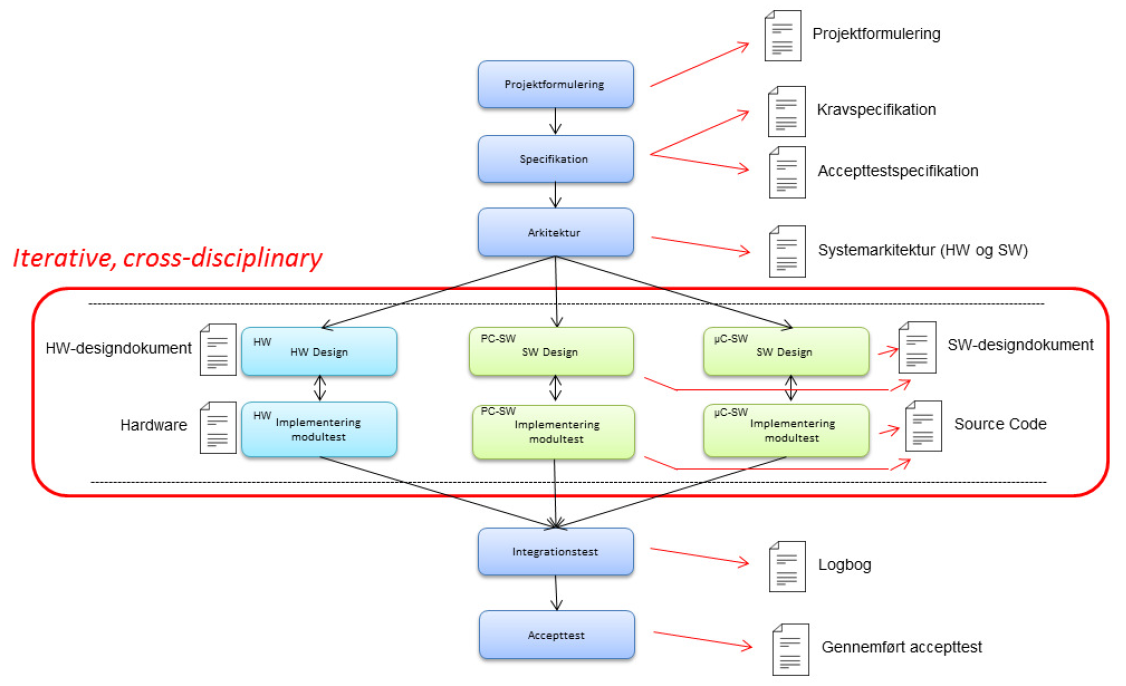
\includegraphics[width=\textwidth]
{Figure/asemodel}}
\caption{V-modellen}
\label{asemodel}
\end{figure}


\begin{figure}[H]
\centering
{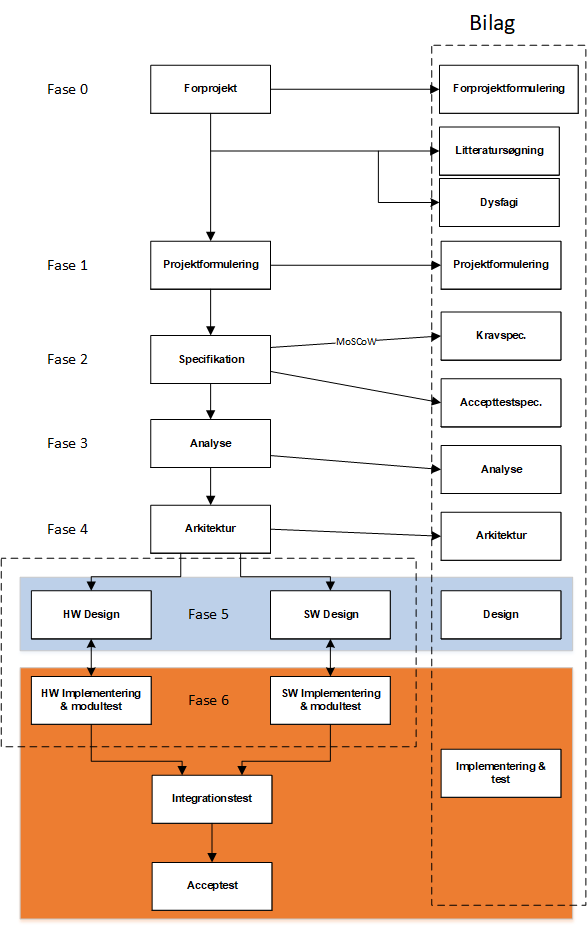
\includegraphics[width=10cm]
{Figure/procesVoresASE}}
\caption{Den modificeret ASE-model.}
\label{procesVoresASE}
\end{figure}





%Udover ASE-modellen blev metoden fra af V-modellen også brugt. Som det kan ses i figur \ref{vmodel} består V-modellen af udviklingsfaser hvor hver fase bliver testet og valideret inden næste fase påbegynder. Dette sikre at man får lavet den højest kvalitet for hver fase og projektet.
%
%Ved udvikling af prototypen blev der er i første fase, udviklet en kravspecifikation fra vores MoSCow analyse. Denne analyse indeholdte alt fra de krav som skulle med i projektet, dem som vi måske kunne nå og dem som vi ikke ville udføre, men kunne perspektivere til og videreudvikles på. Til disse krav blev der forbedret en accepttest, som skal teste det færdige produkts funktioner og egenskaber.
%
%Anden fase er system design. Hvor der undersøges hvilke hardware komponenter som kan bruges til understøtte kravene. Hertil laves en system test, som tester sammenspillet mellem de forskellige systemer efterhånden som de bliver integreret. 
%
%Tredje fase:\\
%fjerde fase:\\
%implementering:\\






\begin{figure}[H]
\centering
{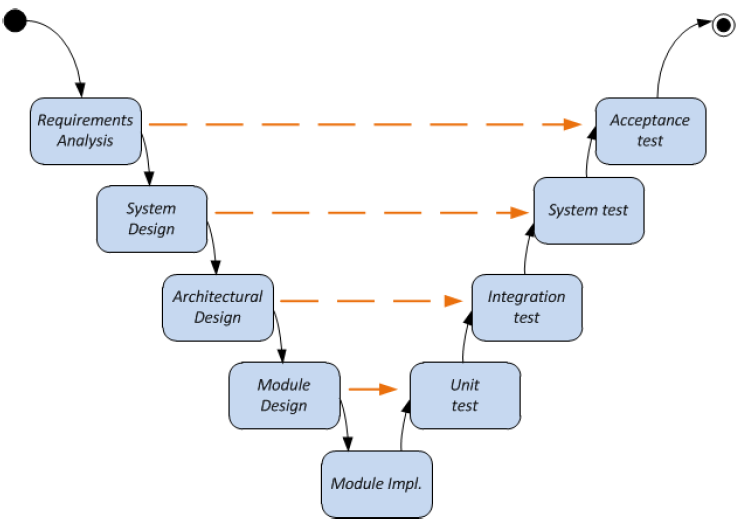
\includegraphics[width=\textwidth]
{Figure/vmodel}}
\caption{V-modellens udviklingsfaser\cite{IngenirhjskolenAarhusUniversitetDevelopmentASE}}
\label{vmodel}
\end{figure}








Til beskrivelse samt opbygning af Synkerefleksmonitor er der fra ISE benyttet metoden SysML. SysML er brugt til diagramanalyse, specifikation, design og verificerer Synkerefleksmonitor. Hvilket resulterer i en beskrivelse af systemets opbygning og kommunikation. Dernæst er der lavet en applikationsmodel, som giver det samlet overblik over Synkerefleksmonitor. Applikationsmodellen består af en domænemodel, hvor alle aktiviterne i synkerefleksmonitor er beskrevet samt tilhørende klassediagrammer med metoder fra sekvensdiagrammer som beskriver systemets virkning og interaktionen mellem de forskellige dele, som er specifikt for hvert use case.\\

Programmet Visio er blevet brugt til udvikling af alle SysML- og UML-diagrammer. Koden og GUI er skrevet og udviklet i Matlab. Rapporten, bilag, mødereferater og logbog er skrevet i tekstsproget Latex på hjemmesiden Overleaf. 

\section{Den gennemførte proces}

Bachelorprojektet startede med at få lavet en tidsplan over hele forløbet, med udkast fra bachelorforprojektet. Her blev der der brugt TeamGantt som projektstyringsværktøj, til oprettelse af tidsplanen, som er en online portal hvor alle gruppedeltager har mulighed for at se og rette i tidsplanen. Siden er bygget op om et Gantt-skeam som viser aktivterne i kalenderformat, som bruges til at dokumenterer planlægningen\cite[s. 297]{IntroductionCompendium}.Ved brug af versionshistorik af tidsplanen, var det muligt at følge ændringer undervejs i projektet. \textit{Se Bilag 2 for versionshistorik af tidsplanen}. Projektet brugte TeamGantt kun til grovplaner med strukturen efter ASE-modellen. Udførelsen af de enkelte elementer fra ASE-modellen blev udført ved brug af V-modellen, for at opretholde en høj kvalitet i projektet. V-modellen sikre at hver fase er færdig og giver mulighed for at test løbende før næste fase begynder\cite[s. 12]{IngenirhjskolenAarhusUniversitetDevelopmentASE}. 




Undervejs er de specifikke opgaver oprettet, for hvert sprint, i programmet Pivotal Tracker. Når en opgave blev oprettet blev der taget op i gruppen hvilken prioritering opgaven skulle have ved brug af en terning fra 1 til 8 point. Hvert medlem viste sine valgte point. Ved uoverensstemmelse af point skulle hvert medlem argumentere og der blev diskuteret i gruppen om en fælles prioritering af opgaven.  






\begin{itemize}
\item SysML og UML
\item Husk referncer til litteratur, samt afvigelser fra teoriens metoder
\end{itemize}

\section{Beskriv Processen 1-2 sider - ikke tekniske del}
\begin{itemize}
\item Gruppedannelser\\
Bachelorprojekt gruppen 




\item Anvendelse af samarbejdsaftaler\\
Der er udarbejdet en samarbjdsaftale som kan ses i Bilag XX. Den er udarbejdet på bag grund af erfaringer fra tideligere projekter og hvad dette projekt kræver.
\item Arbejdsfordeling\\
Arbejdsfordelingen af de praktiskeopgaver og ansvarlige områder er beskrevet i samarbejdsaftalen. se bilag XX. Alle opgaver har været lagt ind i Pivotal Tracker hvor hvert medlem har kunne vælge opgaver efter interesse og efter den overordnet planlægning.
\item Planlægning\\
Teamgantt er den overordnet planlægning som bliver diskuteret og redigeret hver fredag efter et sprint er fuldendt.  
\item Møder\\
Scrum møder hver dag kl. 8:30 som omhandler igangværende opgaver og status og fremgangen på disse. Møde hver fredag. 14 omhandlende ugens sprint og status sprintes opgaver. 
\item Projektledelse\\
Der er en ligefordelt ledelse i gruppen, med et fælles ansvar, med roller, opgave planlægning og organisering. Se samarbejdskontrakt bilag XX.

\item Projektsadministation\\
Der er opdelt ansvarsopgaver i gruppen i mellem såsom, dokument ansvar og referant ved møder. Se den nærmere oversigt i samarbejdsaftalen Bilag XX.
\item Sprints (Scrum)\\
Gruppen har valgt at køre med ugentlige scrum sprints med værktøjet Pivotal Tracker. 
\end{itemize}
Den gennemførte proces beskrives nærmere i procesbeskrivelsen i projektets bilag.


